\begin{figure}[t]
\centering
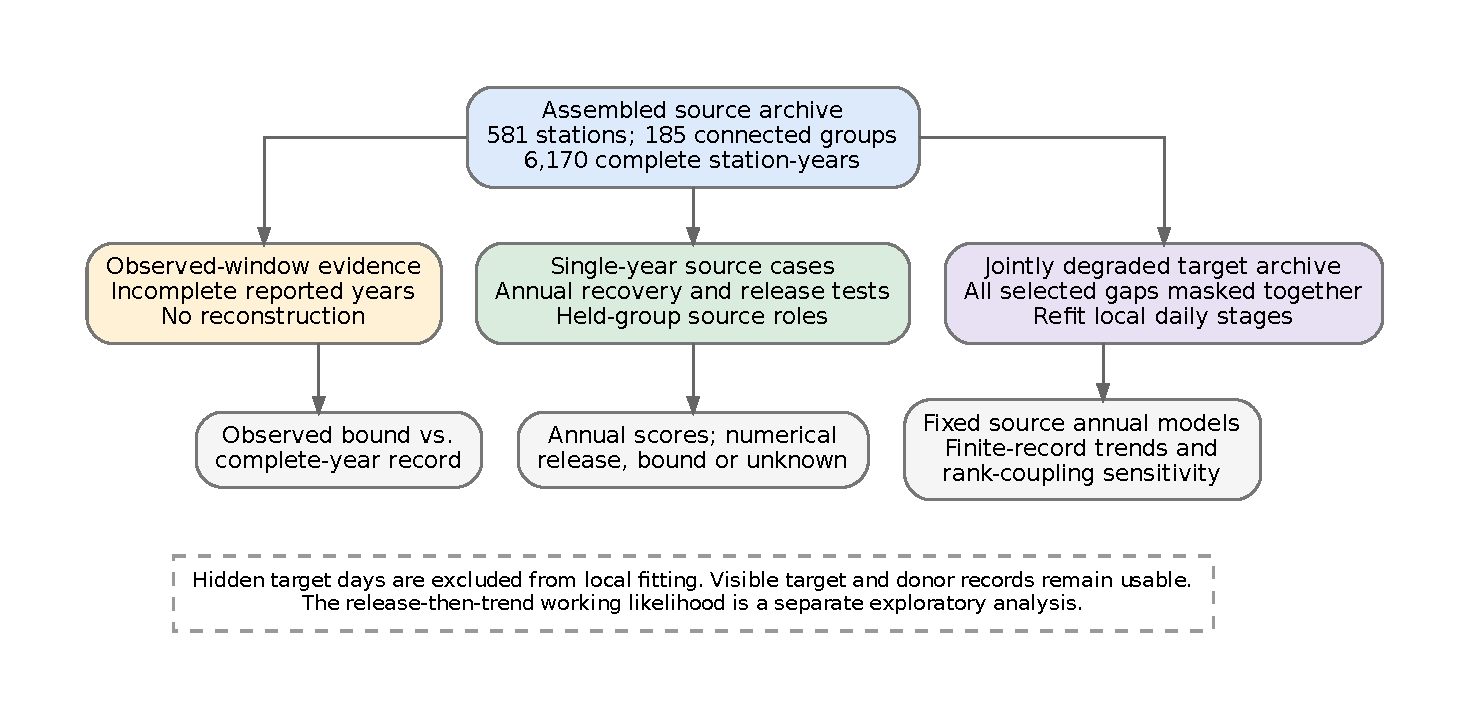
\includegraphics[width=\linewidth]{../wrr_tr/figures/architecture/fig1_evidence_actual.pdf}
\caption{Evidence layers in the leakage-safe benchmark. Observation-only witnesses test whether an incomplete year contains a fully observed 30-day window above the complete-year record; single-year source cases evaluate annual recovery and release; jointly degraded archives mask every selected target year before any local fit and score finite-record trends. Hidden target days never enter the local fit. Takeaway: separating observation-only, annual and whole-archive evidence keeps evaluation quantities out of fitting and selection.}
\label{fig:architecture}
\end{figure}

\begin{figure}[t]
\centering
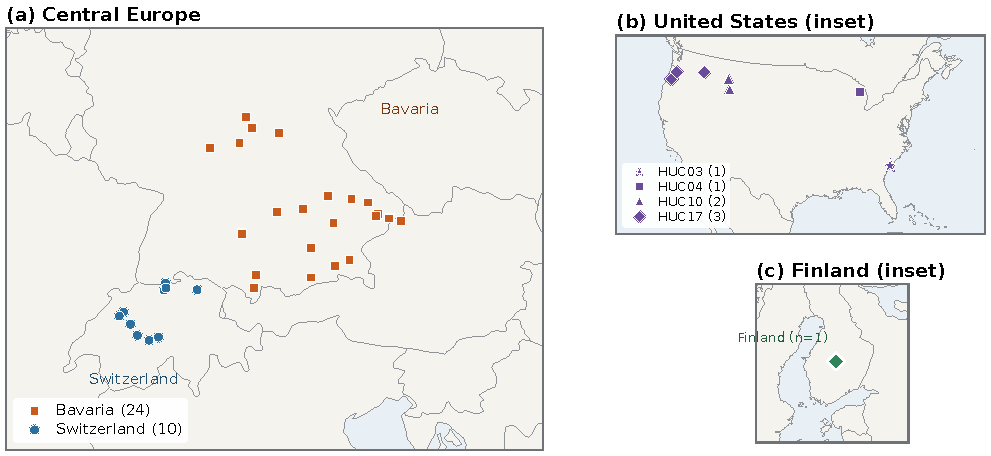
\includegraphics[width=\linewidth]{figures/study_stations.pdf}
\caption{Study-station locator map. The forward cohort contains 24 Bavarian and 10 Swiss stations in Central Europe (a), seven USGS stations in four HUC regions (b), and one Finnish reference site (c) that is not used in forward scoring. Country outlines are Natural Earth 1:50m; this is a locator map, not a basis for area, elevation or discharge covariates. Takeaway: the long-complete cohort is concentrated in Bavaria and Switzerland and is a monitoring-network sample, not a random river sample.}
\label{fig:sample}
\end{figure}

\begin{figure}[t]
\centering
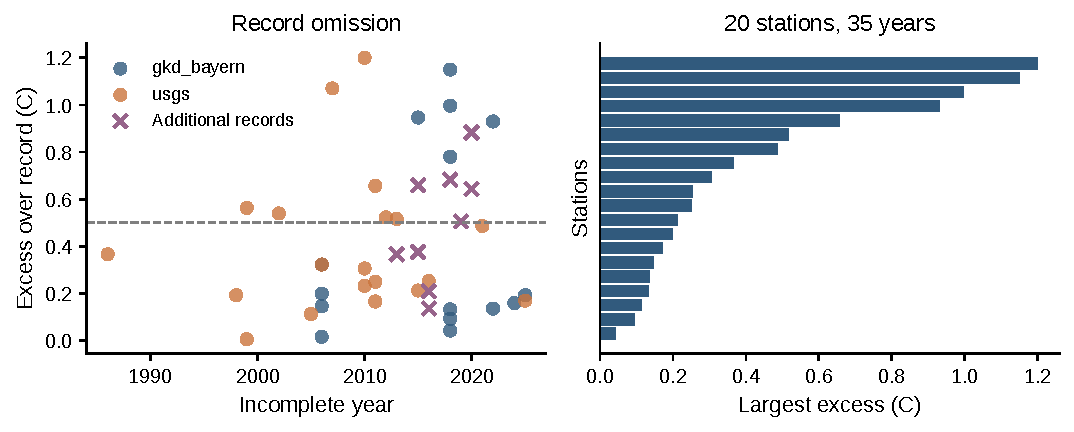
\includegraphics[width=\linewidth]{../wrr_tr/figures/simple_research/01_observed_records.pdf}
\caption{Observed heat evidence discarded by completeness screening. Left: largest fully observed 30-day window above the complete-year H30 record for each incomplete year; right: per-station maximum excess. Crosses are additional approved-record witnesses with sparse complete support and are not in the long-record denominator. Takeaway: 35 incomplete station-years at 20 stations contain observed windows above every complete-year H30, so a completeness screen is not evidence that heat information is absent.}
\label{fig:observed}
\end{figure}

\begin{figure}[t]
\centering
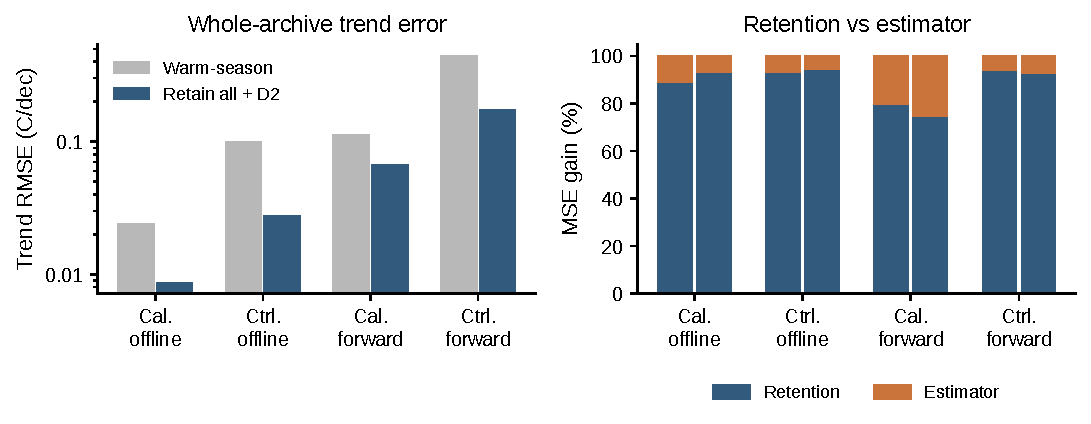
\includegraphics[width=\linewidth]{../wrr_tr/figures/simple_research/03_archive_factorial.pdf}
\caption{Whole-archive trend error and the retention/estimator decomposition. Left: trend RMSE on common station-repetition rows for warm-season screening and all-year recovery under D2, with archive and station/group counts. Right: percentage MSE gain from retention and estimator changes; paired bars use each method's own four-cell count. Takeaway: all-year recovery lowers the absolute slope error in 630 of 805 controlled-gap archives, raises it in 169 and leaves 6 numerically unchanged, so the aggregate gain is not universal.}
\label{fig:trend}
\end{figure}

\begin{figure}[t]
\centering
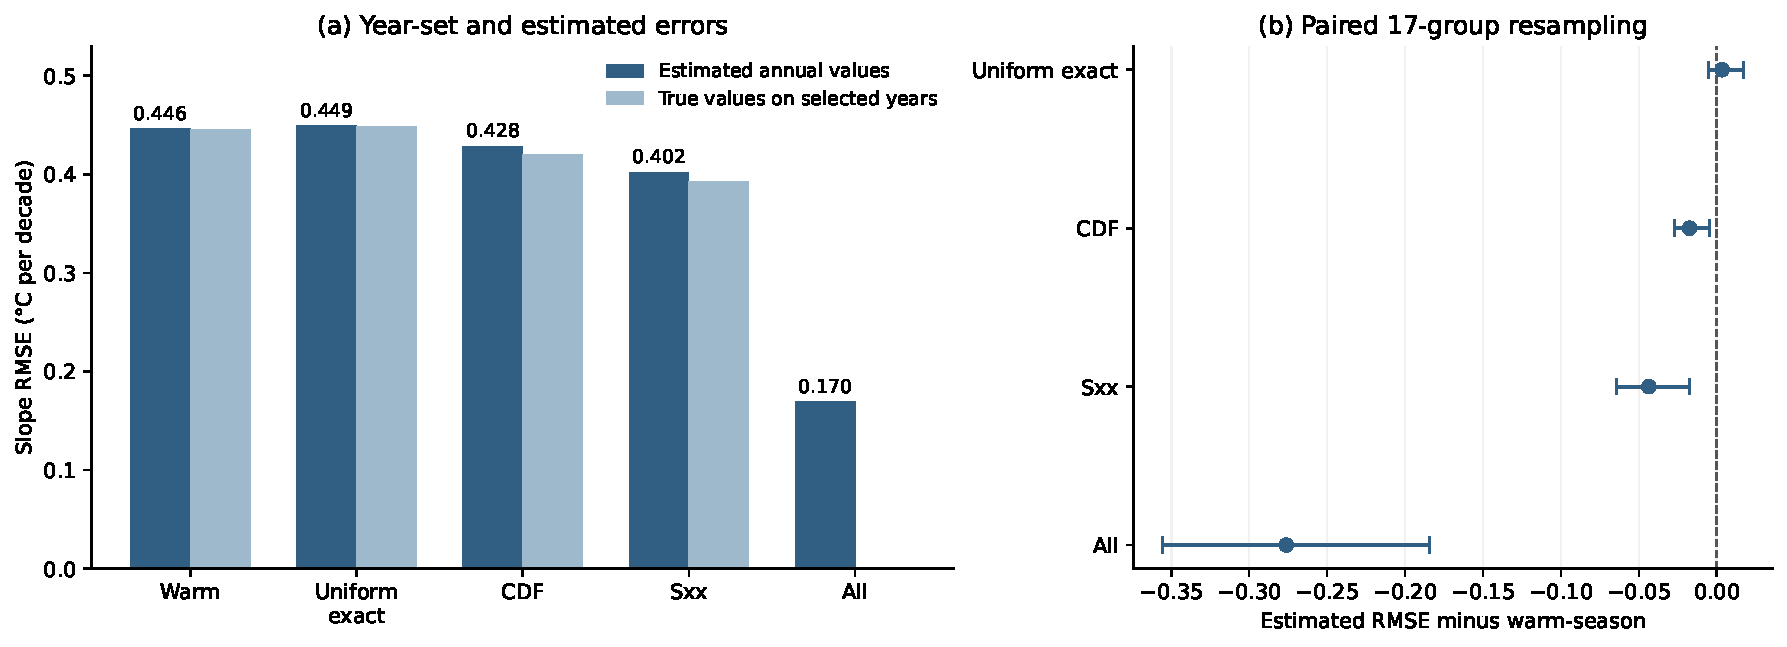
\includegraphics[width=\linewidth]{../wrr_tr/figures/process_revision/03_time_support.pdf}
\caption{Fixed-count year selection on 805 controlled-gap archives. Left: slope RMSE for warm-season screening, uniform exact subset averaging, CDF and $S_{xx}$ selection, using estimated annual values and complete-year H30 on the same selected years; all-year recovery is the reference. Right: comparator-minus-warm-season RMSE differences with paired 95\% percentile intervals from 10{,}000 resamples of 17 connected groups. Takeaway: CDF and $S_{xx}$ improve on warm-season screening at a fixed count, but all-year recovery remains closer to the complete-record slope (0.170 versus 0.428 and 0.402\,$^{\circ}$C/10a).}
\label{fig:selection}
\end{figure}

\begin{figure}[t]
\centering
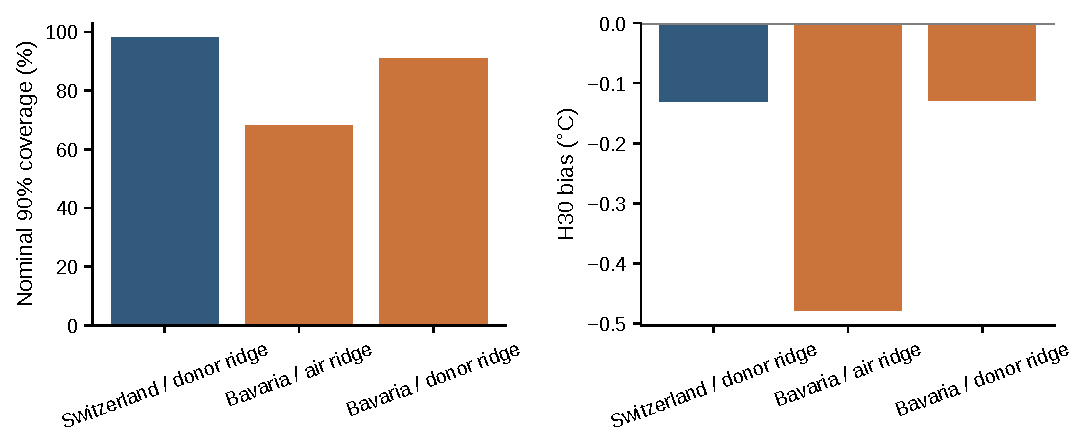
\includegraphics[width=\linewidth]{../wrr_tr/figures/process_revision/02_region_recovery.pdf}
\caption{Hidden-peak recovery by region and daily reconstructor. Left: nominal 90\% interval coverage; right: median bias (recovered minus complete-year H30). Bavarian air-ridge intervals cover 67.9\% of hidden peaks with a $-0.479$\,$^{\circ}$C bias, versus 90.8\% (Bavaria) and 98.1\% (Switzerland) for donor ridges; cases are not matched across reconstructors. Takeaway: recovery fails where local water information is absent, not merely where the calendar rule is imperfect.}
\label{fig:failure}
\end{figure}

\begin{figure}[t]
\centering
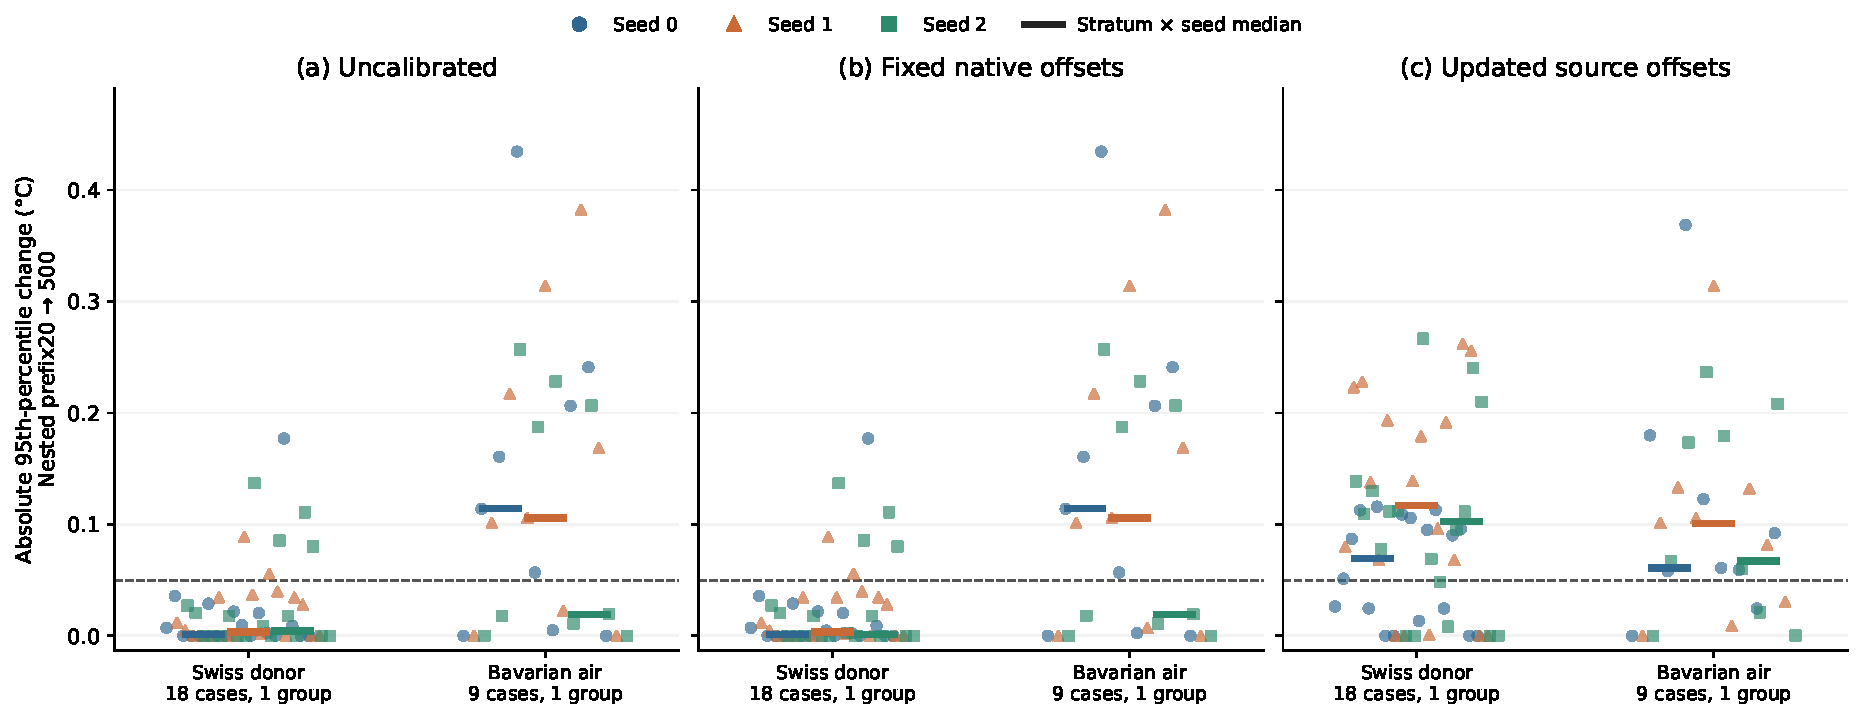
\includegraphics[width=\linewidth]{../wrr_tr/figures/process_revision/04_trajectory_budget.pdf}
\caption{Numerical sensitivity to the residual-bridge budget. Absolute change in the 95th-percentile endpoint between nested 20- and 500-path runs for the same 27 target cases under uncalibrated, fixed-offset and re-estimated-offset settings; colors are seeds and horizontal marks are stratum medians. The 0.05\,$^{\circ}$C line is a numerical diagnostic. Takeaway: the 20-path budget is a numerical-error floor; 500 paths on two target groups establish neither convergence nor a preferred estimator.}
\label{fig:budget}
\end{figure}
